
\subsection{Corruptions}  
    For practical reasons it is important to not only evaluate the models on high-quality data exclusively, but also to know how the predictions will degrade when the input's data quality decreases. Having a model for fluorescence \textit{in silico} labeling that can additionally alarm end users when the predictions should not be relied upon is very useful in practice. Although the DIC microscopy is a relatively easy technique, there are still setting up procedures taking place that can be prone to errors. Additionally, as the models are not easily generalizable across phenotypes as well as between fixed and not fixed cells, an alarming system that is able to catch these situations would be useful to save time and cost of lab work. In order to measure the stability or robustness of the models towards data degeneration they were evaluated on the corrupted or "bad" input DIC images. There are two sources of "bad" images that can be used for such estimations. The first are actually corrupted images made in the laboratory. Such corruptions may come from different sources: for example, an oil bubble landed on the microscope lenses, low density of the cell on the image, over- or underexposure during image acquisition. Another source of image corruption would be images with artificial or pseudocorruptions created manually via image processing. They allow more systematic investigation of the impact of a corruption effect. Artificial corruptions allow to vary the severity of the corruption keeping the original fluorescence data intact.
    
    %This chapter first provides a description of artificial corruptions used to evaluate previously trained models on. Afterwards the real examples of corruptions acquired from the lab are 
    \subsubsection{Artificial corruptions}
        
In this subsection results from evaluating models on 3 types of artificial image corruption are presented, namely: defocus blur imitating the defocus of the microscope lenses, changes in brightness and changes in contrast. Every corruption  has different effects on the prediction of the model based on its severity level. Therefore it is important to evaluate the error-rate (in this case a loss function) for the predictions for different severity levels of each of corruption types presented. It is also important to perform a visual evaluation of model's predictions on corrupted data. Each corruption $c$ will have different severity levels $s$, $-5 \leq s \leq 5$ ($0 \leq s \leq 5$ for defocus blur corruption), where $0$ corresponds to original image without corruption. It is important to keep in mind that although severity levels were chosen to be as much comparable between each other as possible, they still might have differences in their strength. For example, contrast has much stronger effect on predictions than brightness changes. Three types of artificial image corruption are presented below.

\subsubsection{Defocus Blur}
Defocus blur corruption imitates the effect of defocus on the microscope. The blur is applied to the image by convolving it with a special defocus kernel. There are two tunable parameters for this corruption type: first one is the readius of the circle in the kernel $r$, and the second one is the blur strength parameter $s$. Examples of the kernel with radius $r$ is shown in the Figure \ref{fig:defocus-blur-kernel}. Such kernel is then simply applied to an image via $cv2.filter2D$ function.

\begin{figure}[htb]
	\begin{center}
		\includegraphics[width=0.2\linewidth]{bilder/stability/defocus-blur-kernel.png}
		\caption{Defocus blur kernel}\label{fig:defocus-blur-kernel}
	\end{center}
\end{figure}

\subsubsection{Brightness}
Different brightness levels are also an important image corruption to test on. Different brightness levels appear often in the dataset during image accquisition. In oder to change the brightness, an image from the RGB format was translated into HSV format, which stands for hue, saturation and value. This is also one of popular formats to represent an image. To make an image brighter or darker, one can simply add or subtract a parameter $s$ in a value channel for each of the pixels correspondingly. This parameter is often called bias. The bigger absolute value of this change the stronger a corruption will be.

\begin{equation}
    \hat{x}_{i, j} = x_{i, j} + s
\end{equation}

\subsubsection{Contrast}
In contrast to adding a constant value pixelwise to an image in order to change a contrast level one can perform a multiplication of an image with another constant $s$. This parameter is often called gain.

\begin{equation}
    \hat{x}_{i, j} = s * x_{i, j}
\end{equation}

For both contrast and brightness changes one can use $cv2.convertScaleAbs()$ from OpenCV library. This method directly accepts gain and bias parameters and clips the image to stay within the allowed values range.

The values of hyperparameters use in corruptions (kernel radius, gain and bias) are streched across the range of severity levels and presented in Table \ref{table:corruption-hyperparameters}.
\begin{table}[H]
    \centering
    \caption{Hyperparameterization for different artificial corruption severities}
        \begin{adjustbox}{width=1\textwidth}
            \begin{tabular}{|l||*{11}{c|}}\hline
                \backslashbox{Corruption}{Severity}
                &\makebox[3em]{-5}
                &\makebox[3em]{-4}
                &\makebox[3em]{-3}
                &\makebox[3em]{-2}
                &\makebox[3em]{-1}
                &\makebox[3em]{0}
                &\makebox[3em]{1}
                &\makebox[3em]{2}
                &\makebox[3em]{3}
                &\makebox[3em]{4}
                &\makebox[3em]{5}
                \\\hline\hline
                Defocus blur (radius) &-&-&-&-&-&0&0.5&1.0&1.5&2&3\\\hline
                Contrast (gain) &3.5&3.0&2.5&2.0&1.5&1&0.9&0.8&0.7&0.5&0.3\\\hline
                Brightness (bias) &-150&-135&-120&-90&-50&0&50&90&120&135&150\\\hline
            \end{tabular}
        \end{adjustbox}
    \label{table:corruption-hyperparameters}
\end{table}

Severity level of $-5$ for contrast represents an highly contrastive image, while $5$ is a very low contrast image. For brightness corruption levels of $-5$ and $5$ correspond to images with very low and high brightness respectively. And defocus blur corruption has only 5 levels of severity from original image (level $0$) to the image with a stronger blur (level $5$).
\begin{figure}[H]
	\begin{center}
		\includegraphics[width=0.5\linewidth]{bilder/corruptions.png}
		\caption{Influence of artificial corruptions on the predictions}\label{fig:artificial-corruptions}
	\end{center}
\end{figure}

One can observe input image change for each of the corruptions along with the change of prediction of nuclei model on these crops. One can clearly notice that model's predictions are quite stable towards different brightness levels and contrast. However, the predictions on the crops are very sensible towards defocus blur corruption: corruptions of levels $1-4$ are almost indistinctable from the original image, yet the model predictions degrade quite soon. This can be explained by fact that training dataset contains quite diverse data in terms of contrast and brightness levels and, as the result, the model is more stable towards these changes. Using defocus blur as an augmentation will help to solve this problem. This will be described in more detail in Section \ref{section:augments-againts-corruptions}.
\begin{figure}[H]
	\begin{center}
		\includegraphics[width=0.5\linewidth]{bilder/corruptions-loss.png}
		\caption{Change of PCC loss for artificial corruptions}\label{fig:corruptions-loss}
	\end{center}
\end{figure}

Additionally, a change in PCC loss is presented in Figure \ref{fig:corruptions-loss}. This is a plot of PCC loss for different artificial corruptions. The loss is increased for stronger severity levels. We can see that in positive direction with defocus blur corruption the model degerates more quickly and that contrast corruptions change prdictions more sever in the negative one.
    \subsubsection{Real corruptions}
        \label{section:real-corruptions}
        Another interesting set of experiments was conducted on the image data that exhibits real corruptions that can happen in the lab due to the wrong settings of the microscopy image acquisition approach. The following data was considered: 
\begin{figure}[htb]
	\begin{center}
		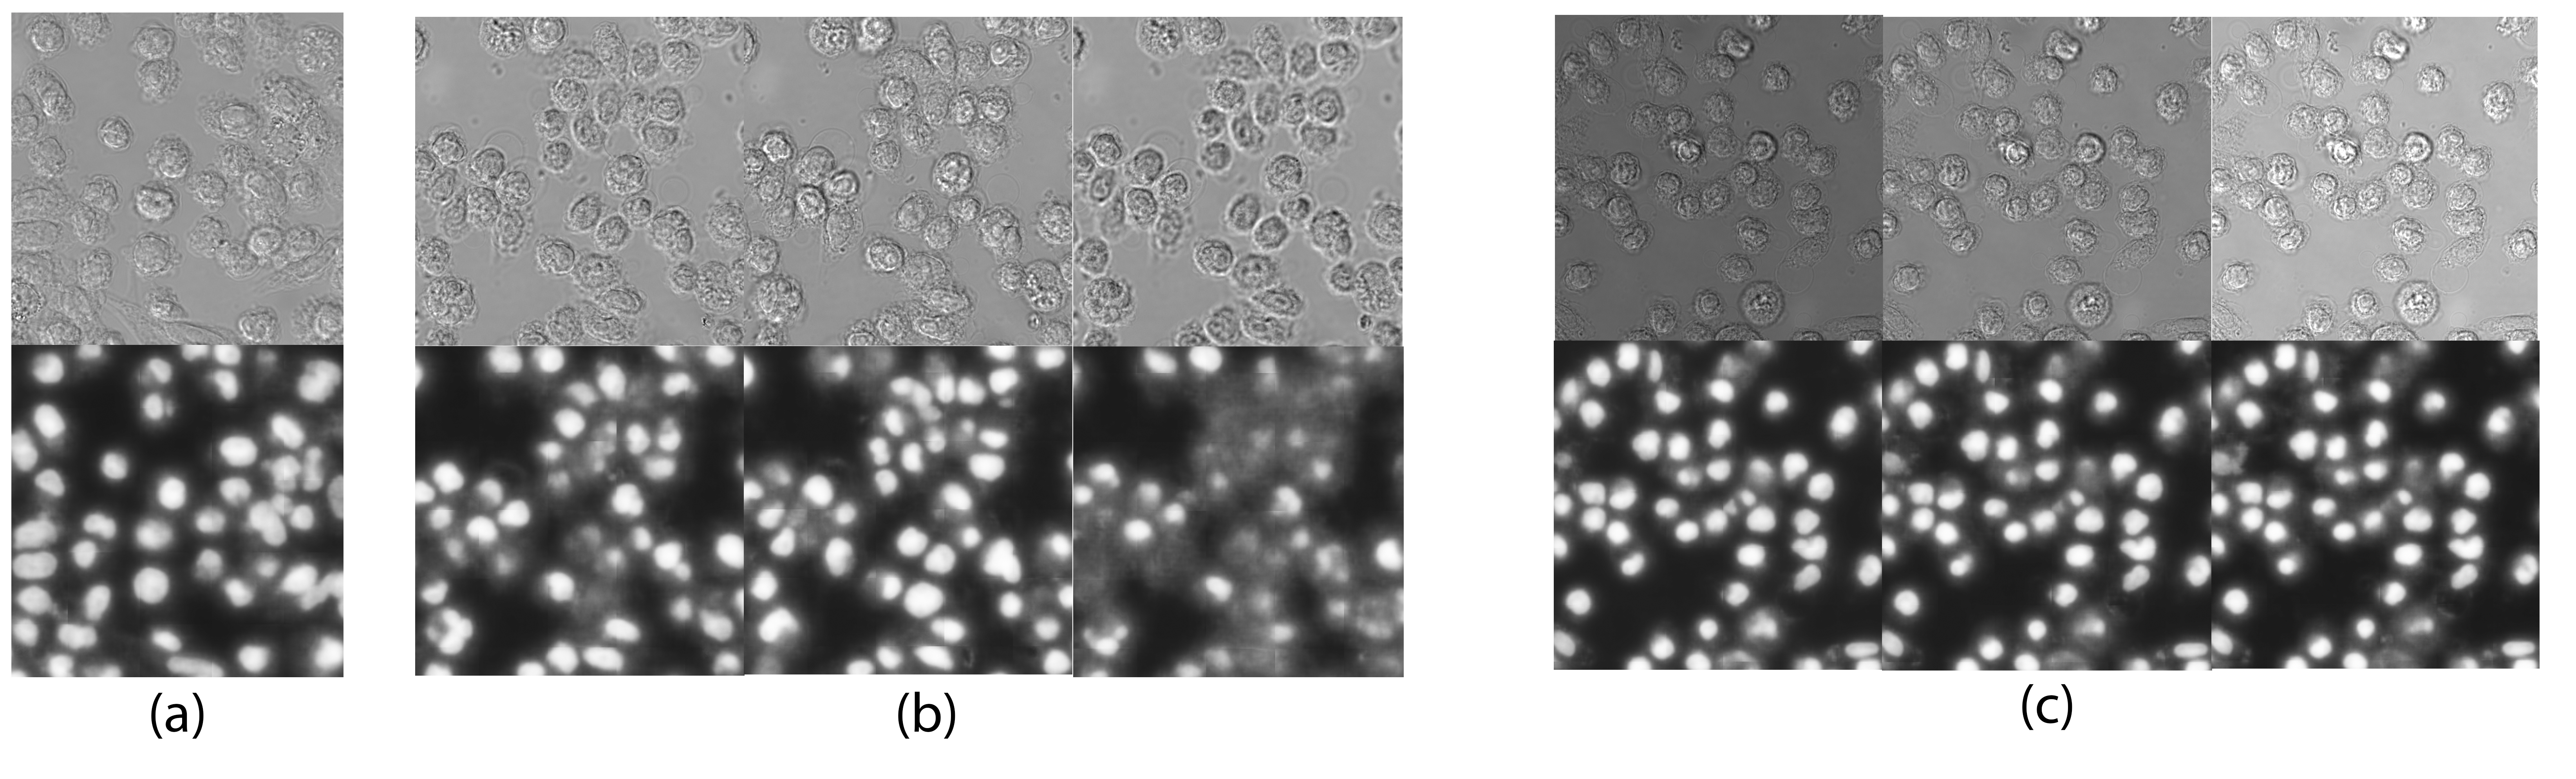
\includegraphics[width=\linewidth]{bilder/drift-detection/real corruptions/predictions.png}
		\caption[]%
		{Real corrupted data from the lab. (a) --- an example of the fixation of the cells in formalin for 15 minutes instead of the usual 10; (b) --- the same image with different microscope focus adjusments. From left to right: microscope stage lowered by 5 microns bringing the subject out of focus, normal height, higher microscope stage by 5 microns bringing the subject out of focus again but in the other direction; (c) --- the same image with different exposure times. From left to right: 20ms --- underexposure, 30ms --- normal setting, 40ms --- overexposure.}\label{fig:real-corruptions-predictions}
	\end{center}
\end{figure}


\begin{itemize}
    \item Figure \ref{fig:real-corruptions-predictions} (a) Wrong fixation time of the cells in formalin. These cells are more turbulent and more strongly clumped together. This is a good example of an image that cannot be simulated artificially with image processing.
    
    \item Figure \ref{fig:real-corruptions-predictions} (b) A real example of a defocus blur from the microscope, when microscope stage was lowered or elevated by 5 microns bringing the subject out of focus.
    
    \item Figure \ref{fig:real-corruptions-predictions} (c) A real example of contrast / brightness differences due to wring exposure times.
\end{itemize}

The model tested here is the model trained on nucleus with simple augmentations (scale, rotation, flips). From Figure \ref{fig:real-corruptions-predictions} it can be concluded that the time of formalin fixing does not really matter for nucleus outline, however the amount of details inside the nuclei seems to be slightly higher than with the usual fixation procedure. Focus of the microscope is clearly very important for good predictions. Although the negative direction of the focus loss seems to have better predictions than the positive one, many of the nuclei are simply gone in the fluorescence image in both cases. Over- and underexposure do not influence the predictions that drastically. Visually different exposure seems to change image brightness and the model is stable towards these changes. Nucleus outline stays mostly the same here as well, but the shining around it is dependent on the exposure times.
    \subsubsection{Improving predictions with additional corruption augmentations}
        \label{section:augments-againts-corruptions}
        \begin{figure}[htb]
	\begin{center}
		\includegraphics[width=0.4\linewidth]{bilder/stability/augments-help.png}
		\caption{Using corruptions as augmentations improves predictions}\label{fig:augments-help}
	\end{center}
\end{figure}

    \subsubsection{Generalizability across phenotypes}
        \label{section:generalizability-across-phenotypes}
        In order to evaluate how well a UNet model is able to generalize across different cell phenotypes the model was first trained on one cell phenotype only and then evaluated on the other cell phenotype. For this experiment CHOZN phenotype was chosen for model training with nuclei fluorescence target, whereas predictions evaluation was performed on PHX phenotype. The predictions were compared with the predictions of the model trained previously on both phenotypes. Comparison was performed both visually and via PCC for the biological metrics. The results in terms of the metrics clearly show the superiority of the model trained on both phenotypes, especially in terms of intensity predictions, where the PCC for the model trained on both phenotypes are almost $3\%$ better. The postprocessing procedures for both models remained the same.

        \begin{table}[H]
            \centering
                \begin{tabularx}{\linewidth}{|Y|YY|}
                    \hline
                    & CHOZN and PHX & CHOZN \\\hline\hline
                    Number of ER & 0.985 & 0.985 \\\hline
                    Total intensity& 0.716 & 0.680\\\hline
                    Mean intensity & 0.732 & 0.708\\\hline
                    Area & 0.986 & 0.960 \\\hline
                \end{tabularx}
                \caption[Generalizability across phenotypes for nuclei predictions]%
                {Generalizability across phenotypes for nuclei predictions. Comparison between the model trained on both phenotypes (CHOZN and PHX) and the model trained on CHOZN cells only in terms of bilogical metrics}
                \label{table:phenotype-generalizability}
        \end{table}
        
        From these results one can notice the general drop in performance on PHX phenotype even for the model that has had PHX cells in training (total intensity PCC for the whole dataset from Table \ref{table:nuclei-downstream-metrics-coefficients} was $0.861$ in comparsion to current $0.716$). The reason for that is generally lower number of PHX samples in nuclei training dataset ($\sim 30\%$).

        Nevertheless, the visual evaluation of the predictions shows little to no difference between predictive models with model trained on both phenotypes giving slightly more details inside the nuclei (see Figure \ref{fig:generalizability}). From this comparsion it was concluded that the model is able to generalize from CHOZN to PHX phentype, however in general PHX phenotype seems to be slightly more challenging for predictions than CHOZN. 

        \begin{figure}[htb]
            \begin{center}
                \includegraphics[width=\linewidth]{bilder/stability/generalizability-phenotypes/only-chozn.png}
                \caption[Visual evaluation of the UNet generalization capabilities]%
                {Visual evaluation of the UNet generalization capabilities. (a) --- ground truth fluorescence of nuclei target of PHX cells, (b) --- prediction of the model trained on both CHOZN and PHX cells, (c) --- prediction of the model trained on PHX cells only}\label{fig:generalizability}
            \end{center}
        \end{figure}